\documentclass{article}
\usepackage[utf8]{inputenc}
\usepackage{mathtools}
\usepackage{amsmath}
\usepackage{amsfonts}
\usepackage{amssymb}
\usepackage{graphicx}
\usepackage[margin=1in]{geometry}
\usepackage{multicol}
\usepackage{enumitem}
\graphicspath{{./img/}}
\setlist{nolistsep}
\setcounter{tocdepth}{2}
\setlength{\columnsep}{1cm}
\title{AP Physics Notes}
\author{Prathmesh Desai}
\date{May 2014}
\begin{document}
\maketitle
\tableofcontents

\newpage
\section{Kinematics}
\subsection{Position, Velocity, and Acceleration}
\begin{multicols}{2}
  \[
  \frac{d\vec{x}}{dt}=\vec{v}(t)
  \]
  \[
  \frac{d^2\vec{x}}{dt^2}=\frac{d\vec{v}}{dt}=\vec{a}(t)
  \]
  \[
  \bar{v}=\frac{\Delta{x}}{\Delta{t}}
  \]
  \[
  \bar{a}=\frac{\Delta{v}}{\Delta{t}}
  \]
  \[
  \vec{v_f}=\vec{v_i}+\vec{a}t
  \]
  \[
  \vec{d}=\vec{v_i}t+\frac{1}{2}\vec{a}t^2
  \]
  \[
  \vec{v_f}^2=\vec{v_i}^2+2\vec{a}(\Delta{x})
  \]
  \[
  g=-9.8\frac{m}{s^2}
  \]
  
  \columnbreak
  
  Free-fall and Projectile Motion:
  \vspace{3mm}
  \begin{itemize}
  \item All free-falling objects do not encounter air resistance\ldots in an ideal world
  \item All free-falling objects (on Earth) accelerate downwards at a rate of approximately $9.8\frac{m}{s^2}$
  \item All free-falling objects have a constant $v_x$
  \item $v_y=0$ \ldots at maximum of y-value of projectile
  \end{itemize}
  
  \vspace{2ex}
  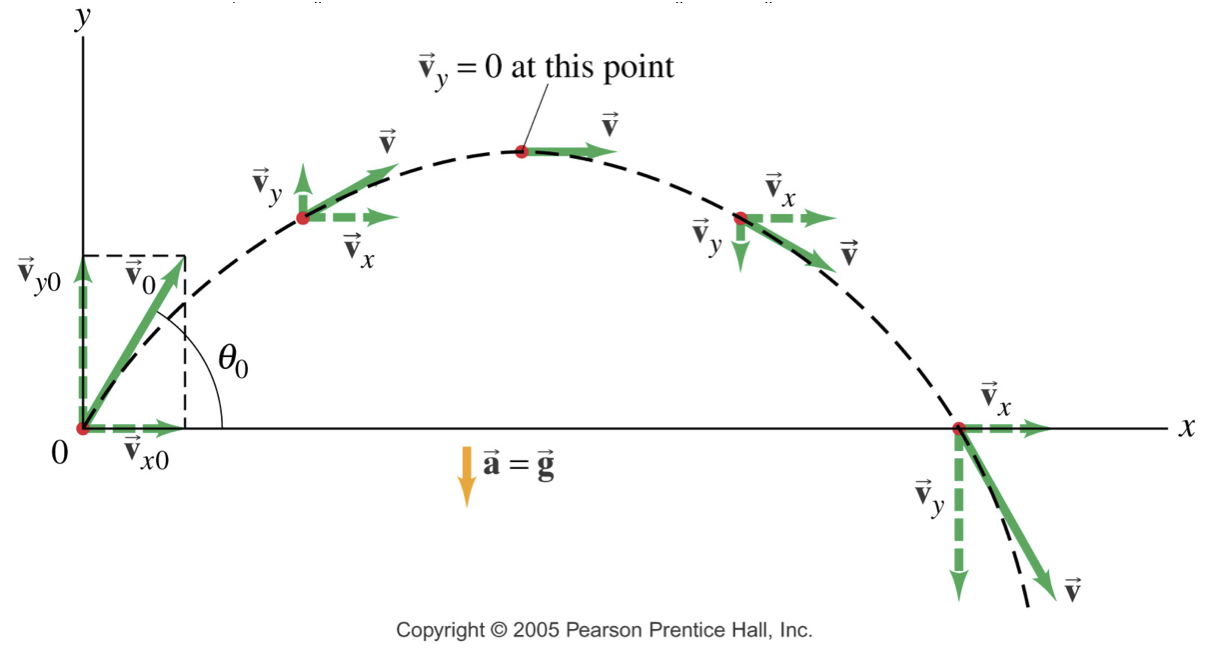
\includegraphics[width=8cm]{ProjectileMotion.jpg}
\end{multicols}
\noindent\textbf{Sample Problems:}
\begin{multicols}{2}
  A loose nail falls from the top of an elevator shaft.  At the same instant 25 m below is the roof of an elevator car rising at a constant 3.0 m/s. \\*\\* Find: \\*
  \begin{enumerate}[label=\alph*]
  \item Position \\*
  \item Velocity of the nail just before it hits the roof of the elevator car\\*
  \end{enumerate}
  Nail: $v_i$ = 0$\frac{m}{s}$ and $d_y$ = 25m, above elevator\\*
  Elevator: $v_i$ = 3$\frac{m}{s}$, up and $d_y$ = 0m
  
  \columnbreak
  
  \textit{In time, $t$, the vertical distance traveled equals:}
  \[
  \Delta{x_n}=25m-\frac{gt^2}{2} \indent \Delta{x_e}=0m-v_et
  \]
  
  \textit{So, $t$ is the solution to the equation:}
  \[
  25m-\frac{gt^2}{2}=0m-v_et \indent t=1.9733s
  \]
  
  \begin{enumerate}[label=\alph*]
  \item $x=v_et=(-3\frac{m}{s})(1.9733s)=19m,$ up \\*
  \item $v_n=gt=(-9.8\frac{m}{s^2})(1.9733s)=19\frac{m}{s},$ down
  \end{enumerate}
  
\end{multicols}

\noindent\centerline{\rule{5cm}{0.4pt}}

\begin {multicols}{2}
  Suppose a volleyball player wants to serve the ball such that it just barely passes over the net.  Let x represent the horizontal distance to the net and y represent the height of the net relative to the launch point of the ball.
  \\*\\*
  Derive an equation that gives the initial launch angle in terms of x and y.
  \columnbreak
  \[
  y=v_i\sin(\theta)t+\frac{at^2}{2} \indent x=v_i\cos(\theta)t
  \]
  \[
  v_i=\frac{y+\frac{gt^2}{2}}{t\sin(\theta)}=\frac{x}{t\cos(\theta)}
  \]
  \[
  y+\frac{gt^2}{2}=\frac{xt\sin(\theta)}{t\cos(\theta)}=x\tan(\theta)
  \]
  \[
  y=\frac{gt^2}{2} \indent y+y=x\tan(\theta) \indent \therefore \theta=tan^{-1}(\frac{2y}{x})
  \]
\end{multicols}

\section{Dynamics}
\subsection{Newton's First Law of Motion}

Every object in a state of uniform motion tends to remain in that state of motion unless an external force is applied to it.
\\\\
\textbf{Inertia}: a property of matter by which it continues in its existing state of rest or uniform motion in a straight line, unless that state is changed by an external force.

\begin{multicols}{2}
  \textbf{For instance} inertia is evident in the famous ``parlor trick'' where the  tablecloth is pulled from under the plates, tumblers, and silverware in a full dining setting. In this case the objects on the table are at rest, and, unless an external force is applied to each individual object, they will remain at rest. When the table cloth is pulled out from under the objects there are no significant external forces in play (friction is negligible if done correctly), and as a result only the tablecloth is removed.
  \columnbreak
  \centerline{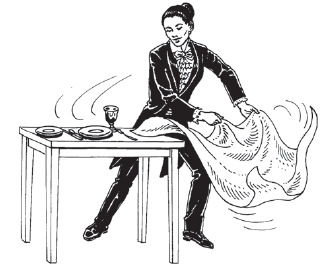
\includegraphics[width=5cm]{tableInertia.png}}
\end{multicols}

\subsection{Newton's Second Law of Motion}

The vector sum of the forces $\vec{F}$ on an object is equal to the mass $m$ of that object multiplied by the acceleration $\vec{a}$ of the object. $\vec{a}$ and $m$ are both directly proportional to $\vec{F}$. The $\vec{F}$ is the vector sum of all \emph{EXTERNAL} forces, so any internal interactions can be ignored.

\[
\Sigma\vec{F}=m\vec{a}
\]

\subsection{Newton's Third Law of Motion}

When one body exerts a force on a second body, the second body simultaneously exerts a force equal in magnitude and opposite in direction on the first body.
\begin{multicols}{2}
  \centerline{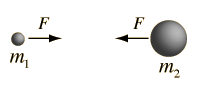
\includegraphics[width=6cm]{thirdLaw.png}}
  \columnbreak
  Without specifying the nature or origin of the forces on the two masses, Newton's 3rd law states that if they arise from the two masses themselves, they must be equal in magnitude but opposite in direction so that no net force arises from purely internal forces.
\end{multicols}

\subsection{Frictional Forces}

The weight of an object is defined as the force of gravity on the object and may be calculated as the mass times the acceleration of gravity.
\[
Weight=F_g=mg \indent g=9.8\frac{m}{s^2}
\]

Frictional resistance to the relative motion of two solid objects is usually proportional to the force which presses the surfaces together as well as the roughness of the surfaces. Since it is the force perpendicular or ``normal'' to the surfaces which affects the frictional resistance, this force is typically called the ``normal force'' and designated by $F_N$.
\[
F_{friction}=\mu F_N
\]
\begin{multicols}{2}
  \noindent$F_N$ is the component of force perpendicular to the surface (surface being a plane) of contact.
  \[
  \mu_s>\mu_k
  \]
  \centerline{$\mu_s$ -- Coefficient of static friction}\\*
  \centerline{$\mu_k$ -- Coefficient of kinetic friction}
  \columnbreak
  \centerline{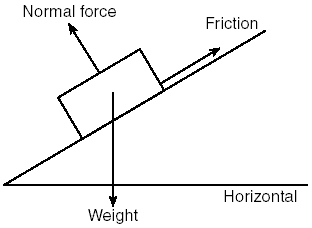
\includegraphics[width=4cm]{normalForce.png}}
\end{multicols}

\subsection{Atwood's Machine}
Friction-less and mass-less pulley:

\begin{multicols}{2}
  \centerline{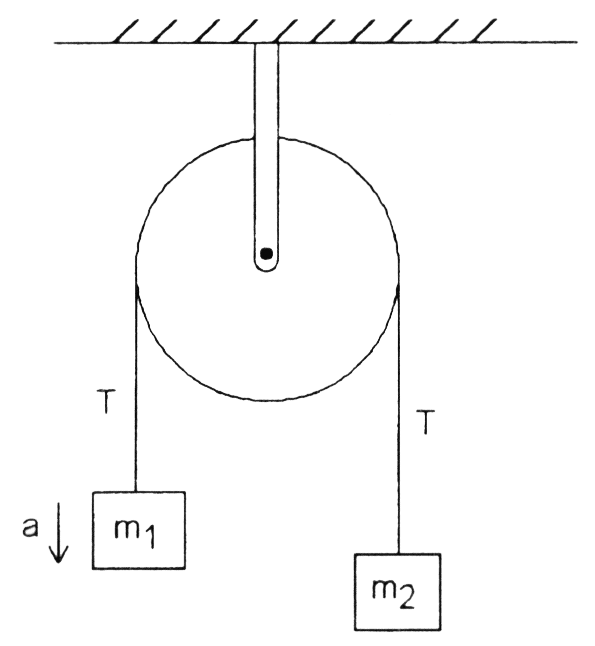
\includegraphics[width=3cm]{atwood.png}}
  \columnbreak
  \[
  m_2>m_1
  \]
  \[
  T=m_1g+\Sigma\vec{F}=m_1g+m_1\vec{a}=m_2g-m_2\vec{a}
  \]
  \[
  m_2g-m_1g-m_1\vec{a}=m_2\vec{a}
  \]
  \[
  \therefore\vec{a}=\frac{g(m_2-m_1)}{m_2+m_1}
  \]
\end{multicols}

\subsection{Air Resistance}
\textbf{Air resistance} is the result of collisions of the object's leading surface with air molecules, and it depends on the speed of the object and the cross-sectional area of the object. Eventually the force of air resistance equals the force of gravity, and prohibits any further acceleration ($\vec{F_{net}}=0$). This state of free-fall is called \textbf{terminal velocity}. Usually it is assumed that air resistance is proportional to speed or that it is proportional to the square of the speed (more accurate).
\[
\vec{F}_{D}\approx -k\vec{v} \indent or \indent \vec{F}_{D}\approx k\vec{v}^2
\indent \text{Force of drag through a fluid: } \frac{1}{2}\rho v^2 C_D A
\]
Air Resistance is demonstrated in the following Position, Velocity, and Acceleration vs. Time graphs:\\
\centerline{
  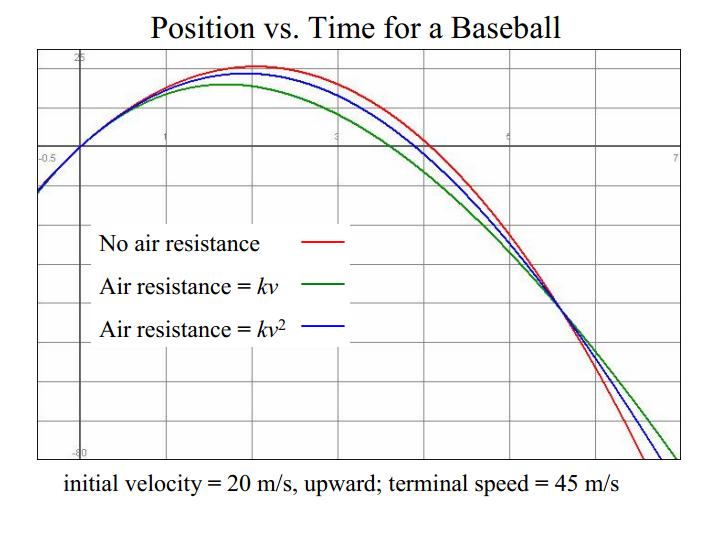
\includegraphics[width=5cm]{pvt_air.png}
  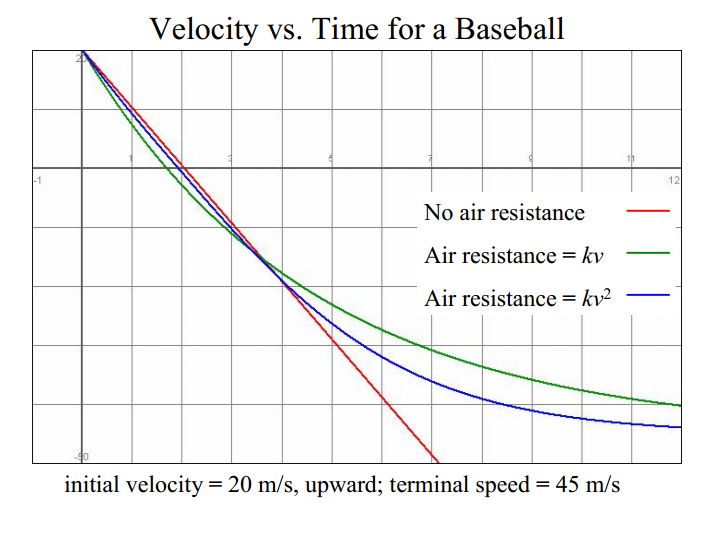
\includegraphics[width=5cm]{vvt_air.png}
  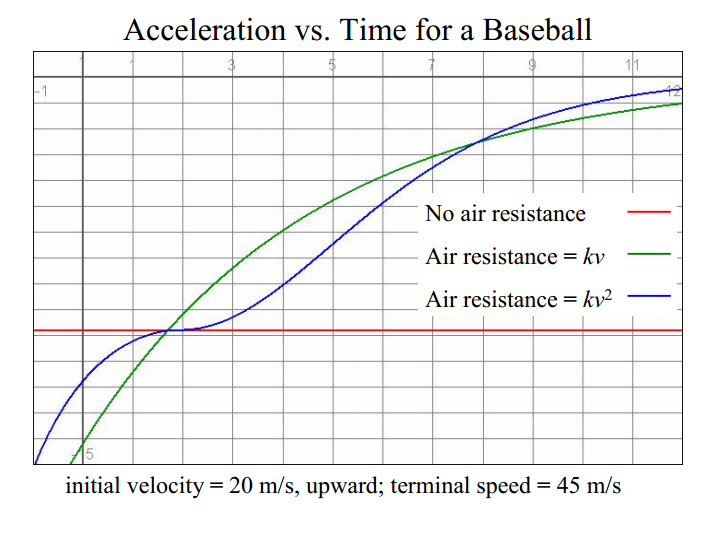
\includegraphics[width=5cm]{avt_air.png}
}
\textbf{Sample Problems:}
\begin{multicols}{2}
  Suppose a baseball of mass $m$ is falling through the air at a velocity $\vec{v}$ that is proportional to drag force $\vec{F}_D$. Solve for $\vec{v}(t)$.
  \[
  \Sigma\vec{F}=m\vec{a}=\vec{F}_g-\vec{F}_D=mg-k\vec{v}
  \]
  Guess and check method:
  \[
  \vec{v}(t)=Ae^{Bt}+C \indent \vec{a}=\frac{d\vec{v}}{dt}=ABe^{Bt}
  \]
  \[
  m\vec{a}=mg-k\vec{v} \indent m(ABe^{Bt})=mg-k(Ae^{Bt}+C)
  \]
  \[
  mABe^{Bt}=mg-kAe^{Bt}-kC
  \]
  \columnbreak
  \[
  0=mg-kC \indent mg=kC \indent C=\frac{mg}{k} \indent \text{(C)}
  \]
  \[
  mABe^{Bt}=-kAe^{Bt} \indent mB=-k \indent B=\frac{-k}{m} \indent \text{(B)}
  \]
  \[
  \vec{v}(t)=Ae^{Bt}+C=Ae^{\frac{-kt}{m}}+\frac{mg}{k}
  \]
  \[
  \vec{v}(0)=Ae^{-k(0)}{m}+\frac{mg}{k} \indent A=\frac{-mg}{k} \indent \text{(A)}
  \]
  \[
  \therefore \indent \vec{v}(t)=\frac{mg}{k}(1-e^{\frac{-kt}{m}})
  \]
\end{multicols}

\noindent\centerline{\rule{5cm}{0.4pt}}

\begin{multicols}{2}
  Must an object always move in the direction of the net force acting upon it?  Explain and give examples to support your answer.
  \vfill
  \columnbreak
  \textit{No, an object doesn't necessarily have to move in the direction of the $\vec{F}_{net}$. An example is circular motion, where the $\vec{F}_{net}$ is towards the center.}
\end{multicols}

\noindent\centerline{\rule{5cm}{0.4pt}}

\begin{multicols}{2}
  A cart on wheels is loaded with books.  In order to move the cart you must exert a relatively great force to start it moving but then a much smaller force to keep it moving.  Use Newton’s laws to explain.
  \vfill
  \columnbreak
  \textit{An object at rest has the tendency to remain at rest, and so the cart loaded with books (when at rest) wants to remain in it's state of rest. Thus, in order to move it one must exert a greater force than the force required to keep the cart in motion.}
\end{multicols}

\noindent\centerline{\rule{5cm}{0.4pt}}

\begin{multicols}{2}
  A pair of fuzzy dice hangs from the ceiling of a car that accelerates forward at $3.00\frac{m}{s^2}$.  Assuming the dice have the same acceleration as the car, what is the angle $\theta$ as shown in the diagram below?\\\\
  \centerline{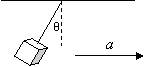
\includegraphics[width=5cm]{dice.png}}
  \columnbreak
  \[
  \Sigma\vec{F}=m\vec{a}=\vec{T}\sin(\theta)
  \]
  \[
  \vec{T}\cos(\theta)=mg \indent \vec{T}=\frac{mg}{\cos(\theta)}
  \]
  \[
  m\vec{a}=\frac{mg\sin(\theta)}{\cos(\theta)}
  \]
  \[
  \frac{\vec{a}}{g}=tan(\theta)
  \]
  \[
  \therefore\theta=tan^{-1}\frac{\vec{a}}{g}=tan^{-1}(\frac{3.00\frac{m}{s^2}}{9.8\frac{m}{s^2}})=17.02^{\circ}
  \]
\end{multicols}

\noindent\centerline{\rule{5cm}{0.4pt}}

\begin{multicols}{2}
  As shown in the diagram below, two blocks are connected by a lightweight cord that passes over a friction-less, mass-less pulley.  The bottom block has a mass of $2.00 kg$ and the top block has mass $0.500 kg$.  The coefficient of kinetic friction at each sliding surface is equal to $0.10$.  The two blocks are release from rest.  Determine the acceleration, $\vec{a}$, of each block.\\\\
  \vfill
  \centerline{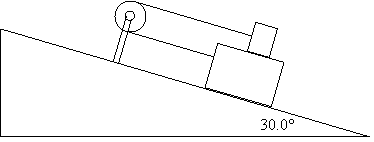
\includegraphics[width=6cm]{frictionPlane.png}}
  \vfill
  \columnbreak
  \noindent\textit{Net force for $m_1$ (smaller block):}
  \[
  \Sigma\vec{F}=m_1\vec{a}=T-m_1 g\sin(\theta)-\mu_km_1g\cos(\theta)
  \]
  \textit{Net force for $m_2$ (larger block):}
  \[
  \Sigma\vec{F}=m_2\vec{a}=m_2g\sin(\theta)-T-\mu_km_1g\cos(\theta)-\mu_k(m_1+m_2)g\cos(\theta)
  \]
  \textit{Solve for $\vec{a}$:}
  \[
  \vec{T}=m_2g\sin(\theta)-\mu_km_1g\cos(\theta)-\mu_k(m_1+m_2)g\cos(\theta)-m_2\vec{a}
  \]
  \[
  T=m_1\vec{a}+m_1 g\sin(\theta)+\mu_km_1g\cos(\theta)
  \]
  \[
  \vec{a}=\frac
      {-g((3m_1+m_2)\cos(\theta)\mu_k+(m_1-m_2)\sin(\theta))}
      {(m_1+m_2)}
      \]
      \[
      \therefore\text{Small Block: }\vec{a}=1.75\frac{m}{s^2} \text{, $150^{\circ}$}
      \]
      \[
      \therefore\text{Large Block: }\vec{a}=1.75\frac{m}{s^2} \text{, $330^{\circ}$}
      \]
\end{multicols}

\section{Circular Motion and Gravity}

\subsection{Uniform Circular Motion}
Anything in circular motion is always accelerating towards the center, this value is called centripetal acceleration. Centripetal means ``center-seeking''. Velocity in circular motion is directed tangential to the circular path of the object.
\begin{multicols}{2}
  \centerline{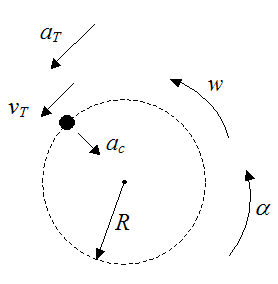
\includegraphics[width=5cm]{circularMotion.png}}
  \columnbreak
  \[
  \vec{v}=\frac{2\pi r}{T}
  \]
  \[
  \vec{a_c}=\frac{v^2}{r}
  \]
  \[
  \Sigma\vec{F}=m(\vec{a_c})=\frac{mv^2}{r}
  \]
  \[
  f=\frac{1}{T}
  \]
\end{multicols}

\textbf{Sample Problem:}
\begin{multicols}{2}
  A car of mass $m$ goes around a curve of radius $r$ banked at an angle of $\theta$ above horizontal. (a) At what speed could the car complete this curve without the aid of lateral friction? (b) Given $\mu_s$ determine the maximum speed at which the car can go around the same curve.
  \centerline{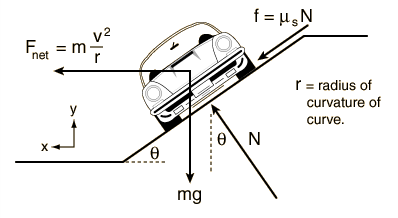
\includegraphics[width=5cm]{bankedCurve.png}}
  Because $\Sigma\vec{F}$ is only in the x-direction we do not need to worry about the y-component.
  \[
  mg=N\cos(\theta)
  \]
  \[
  N=\frac{mg}{cos(\theta)}
  \]
  \[
  N_x=N\sin(\theta)=mg\tan(\theta)
  \]
  \[
  -N=\Sigma\vec{F}=\frac{-mv^2}{r}
  \]
  \[
  g\tan(\theta)=\frac{v^2}{r}
  \]
  \[
  \therefore \vec{v}=\sqrt{rg\tan(\theta)}
  \]
  \vfill
  \columnbreak
  \noindent{y-direction ($\Sigma\vec{F}=0$):}
  \[
  N\cos(\theta)-mg-f\sin(\theta)=0
  \]
  \[
  N\cos(\theta)-\mu_sN\sin(\theta)=mg
  \]
  \[
  N=\frac{mg}{\cos(\theta)-\mu_s\sin(\theta)}
  \]
  x-direction($\Sigma\vec{F}=\frac{mv^2}{r}$)
  \[
  -f\cos(\theta)-N\sin(\theta)=-\frac{mv^2}{r}
  \]
  \[
  N(\sin(\theta)+\mu_s\cos(\theta))=\frac{mv^2}{r}
  \]
  \[
  N=\frac{mv^2}{r(\sin(\theta)+\mu_s\cos(\theta))}
  \]
  Solve for $\vec{v}$:
  \[
  N=\frac{mg}{\cos(\theta)-\mu_s\sin(\theta)}=\frac{mv^2}{r(\sin(\theta)+\mu_s\cos(\theta))}
  \]
  \[
  \therefore \vec{v}=\sqrt{rg(\frac{\sin(\theta)+\mu_s\cos(\theta)}{\cos(\theta)-\mu_s\sin(\theta)})}
  \]
\end{multicols}

\subsection{Parametric Equations}
When a situation is two- or three-dimensional (which is essentially all the time), the position/velocity/acceleration can be determined using parametric equations. Parametric equations are basically equations (shocker!) that describe the behavior of the components of the object, rather than the vector sum of the components.
\[
r_x=x(t) \hspace{1ex} \hat{i} \indent
r_y=y(t) \hspace{1ex} \hat{j} \indent
r_z=z(t) \hspace{1ex} \hat{k} \indent
\]
\[
v_x=\frac{dx}{dt} \hspace{1ex} \hat{i} \indent
v_y=\frac{dy}{dt} \hspace{1ex} \hat{j} \indent
v_z=\frac{dz}{dt} \hspace{1ex} \hat{k}
\]
\[
a_x=\frac{dv_x}{dt}=\frac{d^2v_x}{dt^2} \hspace{1ex} \hat{i} \indent
a_y=\frac{dv_y}{dt}=\frac{d^2v_y}{dt^2} \hspace{1ex} \hat{j} \indent
a_z=\frac{dv_z}{dt}=\frac{d^2v_z}{dt^2} \hspace{1ex} \hat{k}
\]
\[
\vec{r}^2=r_x^2+r_y^2+r_z^2
\]
\[
\vec{v}^2=v_x^2+v_y^2+v_z^2
\]
\[
\vec{a}^2=a_x^2+a_y^2+a_z^2
\]

\subsection{Non-uniform Circular Motion}
Non-uniform circular motion is any case in which an object moving in a circular path has a varying speed. The tangential acceleration is non-zero; the speed is changing.The net acceleration is no longer pointing towards the center, so there are two components of acceleration that we would need to account for:\vspace{1ex}
\begin{multicols}{2}
  \centerline{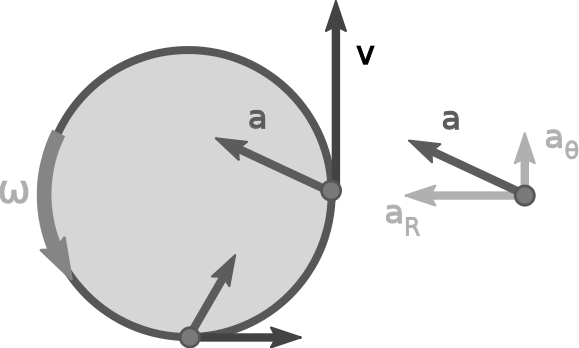
\includegraphics[width=6cm]{noncirc.png}}
  \columnbreak
  \begin{enumerate}
  \item Radial/centripetal acceleration ($a_R$)
  \item Tangential acceleration ($a_\theta$)
  \end{enumerate}
  \[
  \lvert\vec{a}\rvert=\sqrt{\vec{a_\theta}^2+\vec{a_R}^2}
  \]
  We note that velocity, tangential acceleration and tangential force all act along the same direction.
  \[
  a_\theta=\frac{dv}{dt}
  \]
\end{multicols}

\noindent\textbf{Sample Problem:}
\begin{multicols}{2}
  A kid plays with a yo-yo of mass $m$ and twirls it in a vertical circle.  The length of the string is $l$.  The kid twirls it just fast enough to keep it moving in a complete circle – this results in a centripetal acceleration of 5.00 $g$ at the lowest point. (a) Find the speed of the yo-yo at the highest point. (b) Find the speed at the lowest point.
  \vfill
  \columnbreak
  \noindent{\textit{Find $v$ at highest point:}}
  \[
  \Sigma\vec{F}=m\vec{a}=mg \indent
  \vec{a}=g
  \]
  \[
  \vec{a}=\frac{v^2}{r} \indent
  v=\sqrt{\vec{a}r}=\sqrt{gr}
  \]
  \textit{Find $v$ at lowest point:}
  \[
  \vec{a}=5g \indent
  v=\sqrt{\vec{a}r}=\sqrt{5gr}
  \]        
\end{multicols}

\subsection{Newton's Universal Law of Gravitation}
Newton's law of universal gravitation states that any two bodies in the universe attract each other with a force that is directly proportional to the product of their masses and inversely proportional to the square of the distance between them.

\[
\vec{F_G}=G\frac{m_1m_2}{r^2} \indent
G=6.674x10^{-11}\frac{Nm^2}{kg^2}
\]

\subsection{Gravitational Field Strength}
A value ($g$) that is the strength of the gravitational field (acceleration due to gravity) at some place given mass $M$ and radius $r^2$ of object producing the field.
\[
g=\frac{GM}{r^2}
\]

\noindent\textbf{Sample Problems:}

\begin{multicols}{2}
  In 1995, the Galileo robotic spacecraft released a probe into Jupiter’s atmosphere.  When traveling at $v_1 \frac{m}{s}$ the $m$ kg-probe’s main chute deployed and slowed it to $v_2 \frac{m}{s}$ in $t$ seconds.\\\\ (a) Find the force of Jupiter’s gravity acting on the probe.\\\\ (b) Determine the force that the cords of the chute had to withstand.
  \columnbreak
  \vfill
  \noindent{Solve for $F_{jupiter}$}
  \[
  F_{jupiter}=G\frac{m_{chute}m_{jupiter}}{r_{jupiter}^2}
  \]
  Solve for $F_T$ exerted by the cords:
  \[
  \Sigma\vec{F}=m\vec{a}=F_T-F_g
  \]
  \[
  m(\frac{\Delta v}{t})=F_T-F_g
  \]
  \[
  F_T=G\frac{m_{chute}m_{jupiter}}{r_{jupiter}^2}+\frac{v_1-v_2}{t}
  \]
\end{multicols}

\noindent{\centerline{\rule{5cm}{0.4pt}}}

\begin{multicols}{2}
  It can be shown that the value of $g$ inside an empty spherical shell is zero at all points inside the shell (no matter how massive the shell).  Suppose the Earth had uniform density.\\\\ (a) Use these two ideas to solve for $g$ inside the Earth. (Inside the Earth, at any point a distance $r$ from the center, only the mass contained in a sphere of radius $r$ has a net gravitational effect.  All mass between $r$ and the surface has a net gravitational effect of zero.)\\\\ (b) Sketch a graph of $g$ versus $r$ extending from $r = 0$ to $r = 2R_E$.\\\\            \centerline{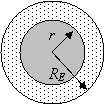
\includegraphics[width=6cm]{p27.png}}
  \vfill
  \columnbreak
  \noindent{Write down equations:}
  \[
  F_g=G\frac{m_1m_2}{r^2} \indent
  g=\frac{GM_E}{r^2}
  \]
  Find ratio of r and $R_E$
  \[
  V_r=\frac{4}{3}\pi r^3 \indent
  V_{R_E}=\frac{4}{3}\pi R_E^3
  \]
  \[
  \frac
      {\frac{4}{3}\pi r^3}
      {\frac{4}{3}\pi R_E^3}
      \indent
      \rightarrow
      \indent
      (\frac{r}{R_E})^3
      \]
      \[
      g=\frac{GM_Er^3}{r^2R_E^3}=\frac{GM_Er}{R_E^3}
      \]
      \[
      g=\frac{r}{R_E}g_{surface}
      \]
      Graph $g$ vs. $r$ from $0$ to $2R_E$\\\\
      \centerline{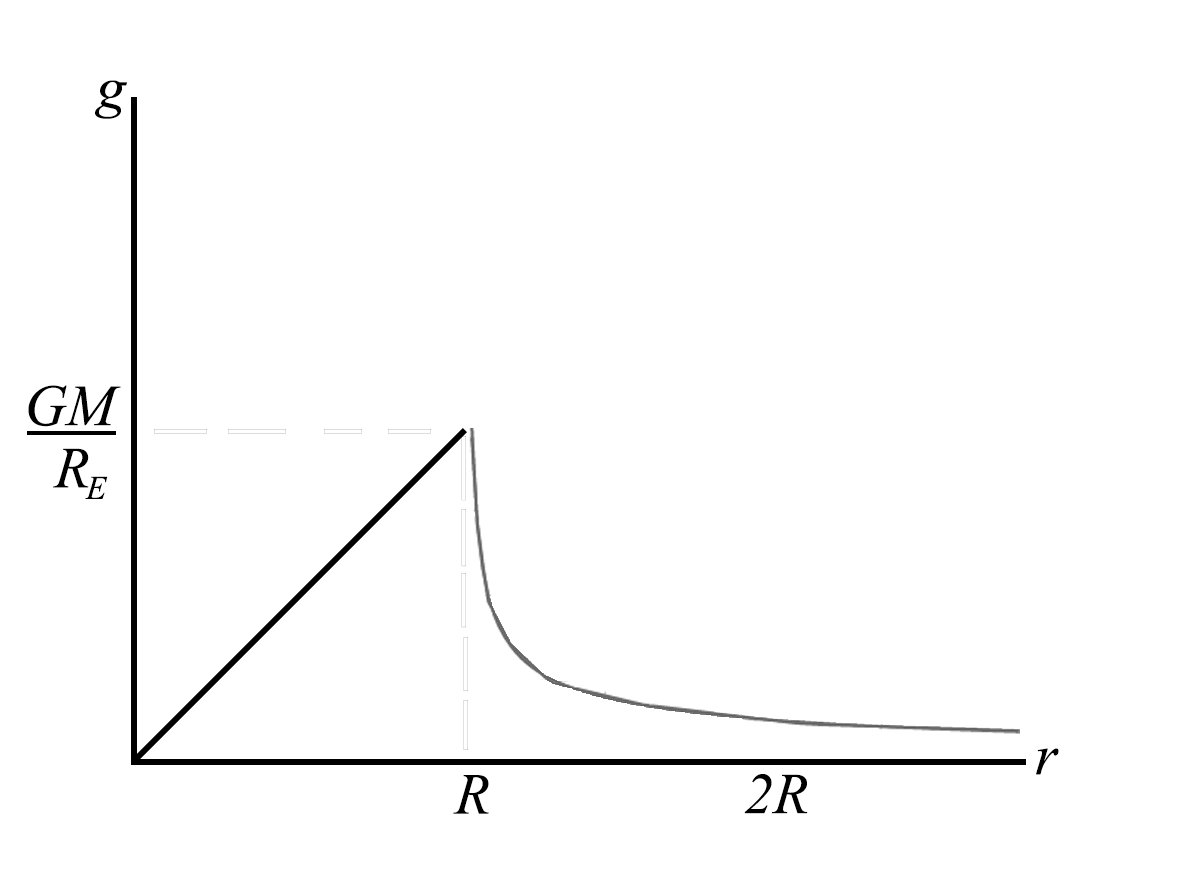
\includegraphics[width=8cm]{graph27.png}}
\end{multicols}

\subsection{Keplar's Laws of Planetary Motion}
In astronomy, Kepler's laws of planetary motion are three scientific laws describing the motion of planets around the Sun.
\vspace{1ex}
\begin{enumerate}
\item The orbit of a planet is an ellipse with the Sun at one of the two foci.
\item A line segment joining a planet and the Sun sweeps out equal areas during equal intervals of time.
\item The square of the orbital period of a planet is proportional to the cube of the semi-major axis of its orbit.
\end{enumerate}
\begin{multicols}{2}
  \centerline{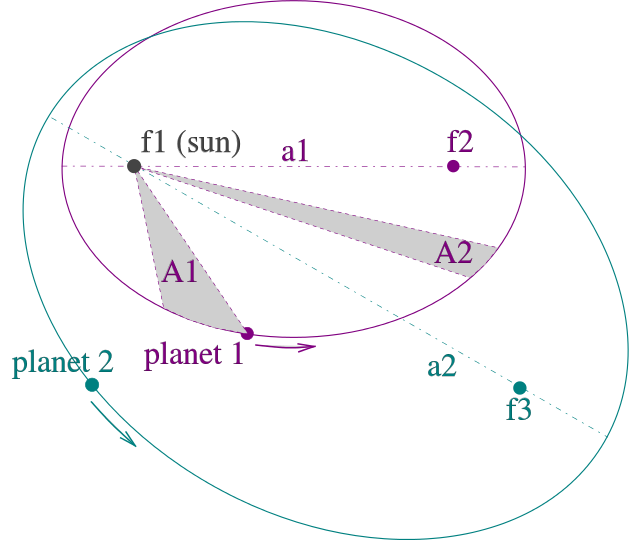
\includegraphics[width=7cm]{keplar.png}}
  \columnbreak
  Keplar's second law is demonstrated by the image, where $A1=A2$ IF they were both swept out in the same amount of time.
  \\\\
  Derive Keplar's Third Law:
  \[
  \vec{F}_c=\vec{F}_g \indent
  \frac{m_2\vec{v}^2}{r}=G\frac{m_1m_2}{r^2}
  \]
  \[
  \vec{v}=\sqrt{\frac{GM}{r}}=\frac{2\pi r}{T}
  \]
  \[
  \frac{r^3}{T^2}=\frac{GM}{4\pi^2} = constant
  \]
  \[
  r^3 \propto T^2
  \]
\end{multicols}

\noindent{\textbf{Sample Problem:}}
\begin{multicols}{2}
  
  Two planets travel in circular orbits around a star.  Planet A has speed $v$ and planet B has speed $3v$.\\\\ (a) Find the ratio of the two planets’ orbital radii.\\\\ (b) Find the ratio of the two planets’ periods.
  \vfill
  \columnbreak
  \noindent{Find ratio of orbital radii:}
  \[
  \frac
      {F_A=\frac{Gm_pm_s}{r_A^2}}
      {F_B=\frac{Gm_pm_s}{r_B^2}}
      \indent
      \frac{r_A}{r_B}=\frac
           {3^2}
           {1^2}
	   \]
	   \[
           \frac{r_A}{r_B}=9
	   \]
	   Find ratio of periods:
	   \[
           \frac
               {T_A^2=r_A^3}
               {T_B^2=r_B^3}
               \indent
               \frac
                   {T_A}
		   {T_B} = \frac{3^3}{1^3}
		   \]
		   \[
             	   \frac{T_A}{T_B}=27
		   \]
\end{multicols}

\section{Work and Energy}
\subsection{Work by Constant and Varying Forces}
When a force acts upon an object to cause a displacement of the object, it is said that \textbf{work} was done upon the object. There are three key ingredients to work - force, displacement, and cause. In order for a force to qualify as having done work on an object, there must be a displacement and the force must cause the displacement.
\\\\
\textbf{Constant Forces} Work is the scalar product of the component of the force in the direction of the displacement and the magnitude of the displacement:
\[
W=Fd\cos(\theta)
\]
\\\\
\textbf{Varying Forces} In a situation with varying force, the particle is displaced in the direction of increasing $x$ from $x_i$ to $x_f$. If we assume $\Delta x$ is an infinitesimal portion of $x$, then $F_x$ would be constant in this displacement. Therefore $\Sigma W$ would be the dot product of $\vec{F}$ and $\vec{r}$:
\[
\Sigma W=\int F\cdot d\vec{r}
\]
\subsection{Work by a String}
If the spring is either stretched or compressed a small distance from its un-stretched (\textit{equilibrium}) configuration, it exerts on the block a force of magnitude (\textit{Hooke's Law}):
\[
F_s=-kx \indent
\text{$x$ is displacement from un-stretched position, and k is the \textbf{spring constant}.}
\]
The negative sign in Hooke's Law signifies that the force exerted by the spring is always directed opposite the displacement. Suppose the block has been pushed to the left a distance $x_{max}$ from equilibrium and is then released:
\[
W_s=\int_{x_i}^{x_f} \vec{F}_s\cdot d\vec{r}=\int_{x_{max}}^0 (-kx)dx=\frac{1}{2} kx_{max}^2
\]

\subsection{Power}
The time rate of doing work is called \textbf{power}. If an external force is applied to an object (which we assume acts as a particle), and if the work done by this force in the time interval $t$ is $W$, then the average power expended during this interval is defined as:
\[
P=\frac{W}{\Delta t}=\frac{dW}{dt}
\]
We find that letting the displacement be expressed as $dr$, that $dW=\vec{F}\cdot d\vec{r}$. Therefore, the instantaneous power can be written:
\[
P_{instantaneous}=\vec{F}\cdot \frac{d\vec{r}}{dt}=\vec{F}\cdot \vec{v}
\]
\[
P_{out}=\text{eff x } P_{in}
\]

\subsection{Kinetic Energy}
Kinetic energy is energy of motion. The kinetic energy of an object is the energy it possesses because of its motion. Kinetic energy is an expression of the fact that a moving object can do work on anything it hits; it quantifies the amount of work the object could do as a result of its motion.
\[
\Sigma W=(\Sigma F)d=(ma)d=m(\frac{v_f-v_i}{t})\frac{1}{2}(v_i+v_f)t=\frac{1}{2}m(v_f^2-v_i^2)
\]
\ldots because work is defined as the change in Kinetic Energy:
\[
KE=\frac{1}{2}mv^2
\]
\[
\Sigma W=\Delta KE=K_f-K_i \indent
\text{Work-Kinetic Energy Theorem}
\]
In a situation where other forces are involved involved, Kinetic Energy is lost or gained. Therefore we would need to modify the Work-Kinetic Energy Theorem to include these forces.
\[
\Delta KE_{friction}=-f_kd
\]
\[
KE_i+\Sigma W_{other}-f_kd=KE_f
\]
\ldots where $\Sigma W_{other}$ represents the sum of the amounts of work done on the object by
forces other than kinetic friction.
\subsection{Potential Energy}
Another form of energy, called \textbf{potential energy} $U$, is the energy associated with a system of objects (two or more objects that exert forces on one another). If the arrangement of the system changes, then the potential energy of the system changes.
\subsubsection{Gravitational Potential Energy}
The product of the magnitude of the gravitational force $mg$ acting on an object and the height $h$ of the object is so important in physics that we give it a name: the \textbf{gravitational potential energy}. The symbol for gravitational potential energy is $U_g$ , and so the defining equation for gravitational potential energy is:
\[
U_g=mgh
\]
Let us now directly relate the work done on an object by the gravitational force to the gravitational potential energy of the object–Earth system. Work is defined as the negative change in potential energy:
\[
W_g=U_i-U_f=-\Delta U_g
\]
Because of the inverse square nature of the gravity force, the force approaches zero for large distances, and it makes sense to choose the zero of gravitational potential energy at an infinite distance away. The gravitational potential energy near a planet is then negative, since gravity does positive work as the mass approaches. This negative potential is indicative of a "bound state"; once a mass is near a large body, it is trapped until something can provide enough energy to allow it to escape. The general form of the gravitational potential energy of mass m is:
\[
U_g=-\int \vec{F}\cdot d\vec{r}=-\int G\frac{Mm}{r^2}r=-G\frac{Mm}{r}
\]
\subsubsection{Elastic Potential Energy}
The elastic potential energy of the system can be thought of as the energy stored in the deformed spring (one that is either compressed or stretched from its equilibrium position). As we have already related Work to both Work of a Spring and Potential Energy we get that:
\[
U_s=\frac{1}{2}kx^2
\]
Also, because the elastic potential energy is proportional to $x^2$, we see that $U_s$ is always positive in a deformed spring.
\begin{multicols}{2}
  \centerline{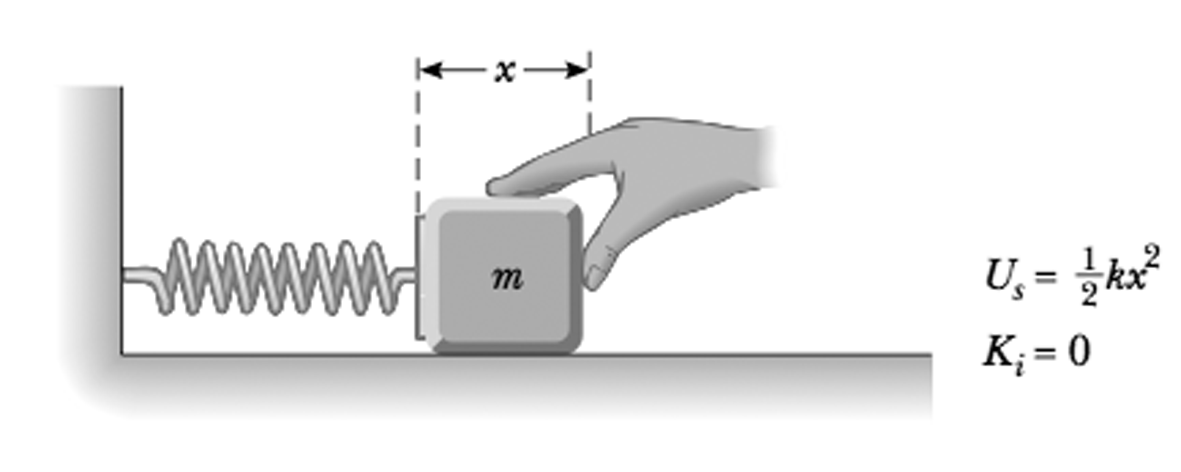
\includegraphics[width=8cm]{p1.png}}
  \columnbreak
  \centerline{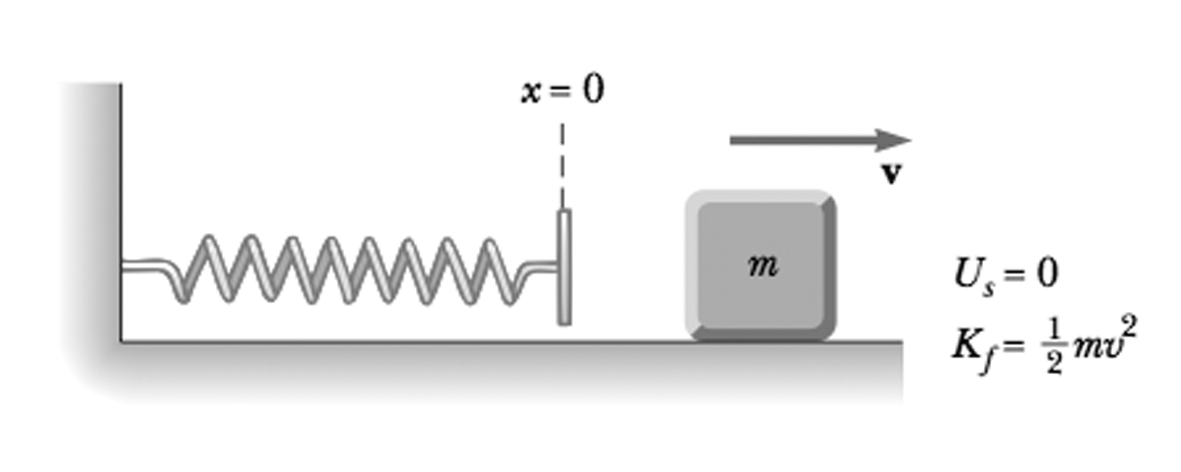
\includegraphics[width=8cm]{p2.png}}
\end{multicols}
\subsection{Conservative and Non-Conservative Forces}
\subsubsection{Conservative Forces}
Conservative forces have two important properties:\\
\begin{enumerate}
\item A force is conservative if the work it does on a particle moving between any two points is independent of the path taken by the particle.
\item The work done by a conservative force on a particle moving through any closed path is zero. (A closed path is one in which the beginning and end points are identical)
\end{enumerate}
The work done by a conservative force equals the negative of the change in the potential energy associated with that force, where the change in the potential energy is defined as $\Delta U=U_f-U_i$:
\[
W_c=-\Delta U
\]
The equation above can also be re-written as:
\[
\Delta U=-\int \vec{F}\cdot d\vec{r} \indent
or \indent
F_x=-\frac{dU}{dx}
\]
\subsubsection{Non-Conservative Forces}
A force is non-conservative if it causes a change in mechanical energy E, 5.3 which we define as the sum of kinetic and potential energies. For example, if a book is sent sliding on a horizontal surface that is not friction-less, the force of kinetic friction reduces the book’s kinetic energy. As the book slows down, its kinetic energy decreases. As a result of the frictional force, the temperatures of the book and surface increase. Experience tells us that this internal energy cannot be transferred back to the kinetic energy of the book. In other words, the energy transformation is not reversible. Because the force of kinetic friction changes the mechanical energy of a system, it is a non-conservative force.
\subsection{Conservation of Energy}
The total mechanical energy of a system remains constant in any isolated system of objects that interact only through conservative forces. Because the total mechanical energy E of a system is defined as the sum of the kinetic and potential energies, we can write:
\[
E=U+K
\]
We can state the principle of conservation of energy as $E_i=E_f$ , and so we have:
\[
U_i+K_i=U_f+K_f
\]
\ldots and if we add Work done by Non-Conservative forces to the Conservation of Energy equation, we get:
\[
W_{NC}+U_i+K_i=U_f+K_f
\]
If non-conservative forces (such as friction) act on objects inside a system, then mechanical energy is not conserved. In these situations, the difference between the total final mechanical energy and the total initial mechanical energy of the system equals the energy transferred to or from the system by the non-conservative forces.

\section{Linear Momentum}
\subsection{Linear Momentum and Conservation}
The linear momentum of a particle of mass $m$ moving with a velocity $v$ is defined to be the product of the mass and velocity:
\[
\vec{p}=m\vec{v}
\]
If a particle is moving in an arbitrary direction, $\vec{p}$ must have three components:
\[
p_x=mv_x \indent
p_y=mv_y \indent
p_z=mv_z
\]
Linear momentum is a vector quantity because it equals the product of a scalar quantity $m$ and a vector quantity $v$. Its direction is along $v$, and its SI unit is $\frac{kgm}{s}$. Using Newton’s second law of motion, we can relate the linear momentum of a particle to the resultant force acting on the particle: The time rate of change of the linear momentum of a particle is equal to the net force acting on the particle:
\[
\Sigma\vec{F}=\frac{d\vec{p}}{dt}=\frac{d(m\vec{v})}{dt}
\]
\subsubsection{Conservation of Momentum for a Two-Particle System}
\begin{multicols}{2}
  \centerline{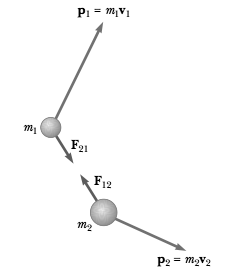
\includegraphics[width=6cm]{conMomentum.png}}
  \columnbreak
  At some instant, the momentum of particle 1 is $\vec{p}_1=m_1\vec{v}_1$ and the momentum of particle 2 is $\vec{p}_2=m_2\vec{v}_2$.Note that $\vec{F}_{12}=-\vec{F}_{21}$. The total momentum of the system $p_{net}$ is equal to the vector sum $\vec{p_1}+\vec{p_2}$.\\
  Because the time derivative of the total momentum $p_{net}=p1+p2$ is zero, we conclude that the total momentum of the system must remain constant:
  \[
  \Sigma\vec{p}=\underset{system}{\Sigma}\vec{p}=p_1+p_2=constant
  \]
  \[
  p_{1i}+p_{2i}=p_{1f}+p_{2f}
  \]
  Whenever two or more particles in an isolated system interact, the total momentum of the system remains constant.
\end{multicols}
\subsection{Impulse}
\textbf{Impulse} is a ``driving force'' that acts on a particle that equals the change in momentum of the particle caused by the force acting on a time interval from $t_i$ to $t_f$. Impulse is a vector defined by:
\[
\vec{J}=\int_{t_i}^{t_f} \vec{F} dt=\bar{F}\Delta t=\Delta\vec{p}
\]
This time-averaged force $(\bar{F})$ used in the equation above can be thought of as the constant force that would give to the particle in the time interval $t$ the same impulse that the time-varying force gives over this same interval.

\subsection{Elastic and Inelastic Collisions}
\subsubsection{Elastic Collisions}
An \textbf{elastic collision} between two objects is one in which total kinetic energy (as well as total momentum) is the same before and after the collision. Billiard-ball collisions and the collisions of air molecules with the walls of a container at ordinary temperatures are approximately elastic. Truly elastic collisions rarely occur in the real world (except on the atomic level). In this case, both momentum and kinetic energy are conserved; therefore, we have:
\[
m_1v_{1i}+m_2v_{2i}=m_1v_{1f}+m_2v_{2f}
\]
\[
\frac{1}{2}m_1v_{1i}^2+\frac{1}{2}m_2v_{2i}^2=\frac{1}{2}m_1v_{1f}^2+\frac{1}{2}m_2v_{2f}^2
\]
In a typical elastic collision problem you will have two unknowns (most of the time it's velocity), and both equations must be used to solve for the unknowns.
\subsubsection{Inelastic Collisions}
Consider two particles of masses $m_1$ and $m_2$ moving with initial velocities $v_{1i}$ and $v_{2i}$ along a straight line. The two particles collide head-on, stick together, and then move with some common velocity $v_f$ after the collision. Because momentum is conserved in any collision, we can say that, in an \textbf{Inelastic Collision}, the total momentum before the collision equals the total momentum of the composite system after the collision\ldots and kinetic energy is not conserved:
\[
v_f=\frac{m_1v_{1i}+m_2v_{2i}}{m_1+m_2}
\]
\subsection{Two-Dimensional Collisions}
In order to analyze two-dimensional collisions we must split the momentum up into components:
\[
m_1v_{1ix}+m_2v_{2ix}=m_1v_{1fx}+m_2v_{2fx}
\]
\[
m_1v_{1iy}+m_2v_{2iy}=m_1v_{1fy}+m_2v_{2fy}
\]
\centerline{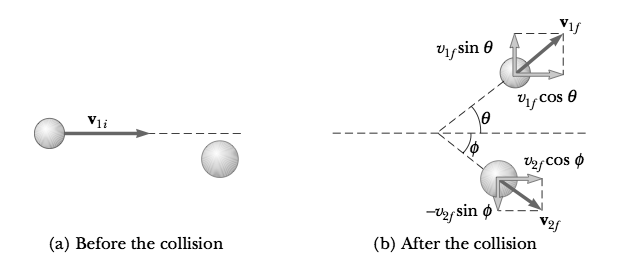
\includegraphics[width=15cm]{collisionP.png}}

\subsection{Center of Mass}
\textbf{Center of Mass} is a point representing the mean position of the matter in a body or system, and it lies on an axis of symmetry and on any plane of symmetry. If the resultant external force on the system is $\vec{F}_{ext}$ and the total mass of the system is $M$, the center of mass moves with an acceleration given by $\vec{a}_{CM}=\frac{\vec{F}_{ext}}{M}$. That is, the system moves as if the resultant external force were applied to a single particle of mass $M$ located at the center of mass. The concept of the center of mass is that of an average of the masses factored by their distances from a reference point. In one plane, that is like the balancing of a seesaw about a pivot point with respect to the torques produced. In one-dimension, the position of the CM is:
\[
x_{CM}=\frac{m_1x_1+m_2x_2+\ldots+m_nx_n}{m_1+m_2+\ldots+m_n}=\frac{\underset{i}{\Sigma}m_ix_i}{\underset{i}{\Sigma}m_i}
\]
\[
y_{CM}=\frac{\underset{i}{\Sigma}m_iy_i}{\underset{i}{\Sigma}m_i}
\]
\[
z_{CM}=\frac{\underset{i}{\Sigma}m_iz_i}{\underset{i}{\Sigma}m_i}
\]
We can also use position vector $\vec{r}$ to locate the Center of Mass, by breaking it into $x_{CM}$, $y_{CM}$, and $z_{CM}$ components.
\[
\vec{r}_{CM}=x_{CM}\textbf{i}+y_{CM}\textbf{j}+z_{CM}\textbf{k}
\]
If we allow $n$ to approach infinity we replace the elements of mass (mass increases as we go along the object) by $dm$ and replace $\underset{i}{\Sigma}m_i$ by $M$, and we get:
\[
\vec{r}_{CM}=\frac{1}{M}\int\vec{r}dm
\]
Because an extended object is a continuous distribution of mass ($dm$), each small mass element is acted upon by the force of gravity. The net effect of all these forces is equivalent to the effect of a single force, $Mg$, acting through a special point, called the \textbf{center of gravity}. If $g$ is constant over the mass distribution, then the center of gravity coincides with the center of mass. If an extended object is pivoted at its center of gravity, it balances in any orientation.

\subsection{Motion of a System of Particles}
The center of mass of a system of particles of combined mass $M$ moves like an equivalent particle of mass $M$ would move under the influence of the resultant external force on the system. The net force on the system of particles is cause only by external forces, thus we get:
\[
\Sigma\vec{F}_{ext}=M\vec{a}_{CM}=\frac{d\vec{p}_{net}}{dt}
\]
Thus, we can also assume that the velocity and acceleration of the Center of Mass equals:
\[
\vec{v}_{CM}=\frac{d\vec{r}_{CM}}{dt}=\frac{\underset{i}{\Sigma}m_i\vec{v}_i}{M}
\]
\[
\vec{a}_{CM}=\frac{d\vec{v}_{CM}}{dt}=\frac{\underset{i}{\Sigma}m_i\vec{a}_i}{M}
\]
If the resultant external force is zero, then:
\[
\vec{p}_{net}=M\vec{v}_{CM}=constant \indent
\Sigma\vec{F}=0
\]

\section{Rotational Mechanics}
\subsection{Angular Displacement, Velocity, and Acceleration}
In dealing with a rotating object, analysis is greatly simplified by assuming that the object is rigid. A rigid object is one that is nondeformable, it is an object in which the separations between all pairs of particles remain constant. All real bodies are deformable to some extent; however, our rigid-object model is useful in many situations in which deformation is negligible. In addition, there are rotational equivalents to the linear values we are so familiar with -- angular displacement ($\theta$), angular velocity ($\omega$), and angular acceleration ($\alpha$) -- and they can be calculated using the following, where $r$ is the radius:
\[
s=r\theta \indent
v=r\omega \indent
a=r\alpha
\]
\[
\omega=\frac{d\theta}{dt} \indent
\alpha=\frac{d\omega}{dt}=\frac{d\theta^2}{d^2t}
\]

\subsection{Rotational Kinematics}
Similar to variable equivalents between angular and linear motion, we also have equivalent kinematic equations for a constant angular acceleration:
\[
\omega_f=\omega_i+\alpha t
\]
\[
\theta_f=\theta_i+\omega_it+\frac{1}{2}\alpha t^2
\]
\[
\omega_f^2=\omega_i^2+2\alpha(\theta_f-\theta_i)
\]
\subsection{Rotational Energy}
Let us now look at the kinetic energy of a rotating rigid object, considering the object as a collection of particles and assuming it rotates about a fixed $z$ axis with an angular speed $\omega$. Each particle has kinetic energy determined by its mass and linear speed. If the mass of the $i$th particle is $m_i$ and its linear speed is $v_i$, its kinetic energy is:
\[
K_i=\frac{1}{2}m_iv_i^2
\]
So, the total kinetic energy of the rotating rigid object is the sum of the kinetic energies of the individual particles, where $K_R$ is the Rotational Kinetic Energy:
\[
K_R=\frac{1}{2}(\Sigma m_ir_i^2)\omega^2
\]
We simplify this expression by defining the quantity in parentheses as the moment of inertia $I$:
\[
I=\Sigma m_ir_i^2 \indent
So\ldots\indent
K_R=\frac{1}{2}I\omega^2
\]

\subsection{Moment of Inertia}
The Moment of Inertia can be calculated by integrating infinitesimal portions of the rigid object, where $r$ is the radius and $dm$ is the infinitesimal mass.
\[
I=\int r^2 dm
\]
It is usually easier to calculate moments of inertia in terms of the volume of the elements rather than their mass. So, we replace mass per unit length, area, or volume by symbols:
\[
\lambda=\frac{m}{L} \indent
\sigma=\frac{m}{A} \indent
\rho=\frac{m}{V}
\]
\textbf{Common Moments of Inertia:}\\
\centerline{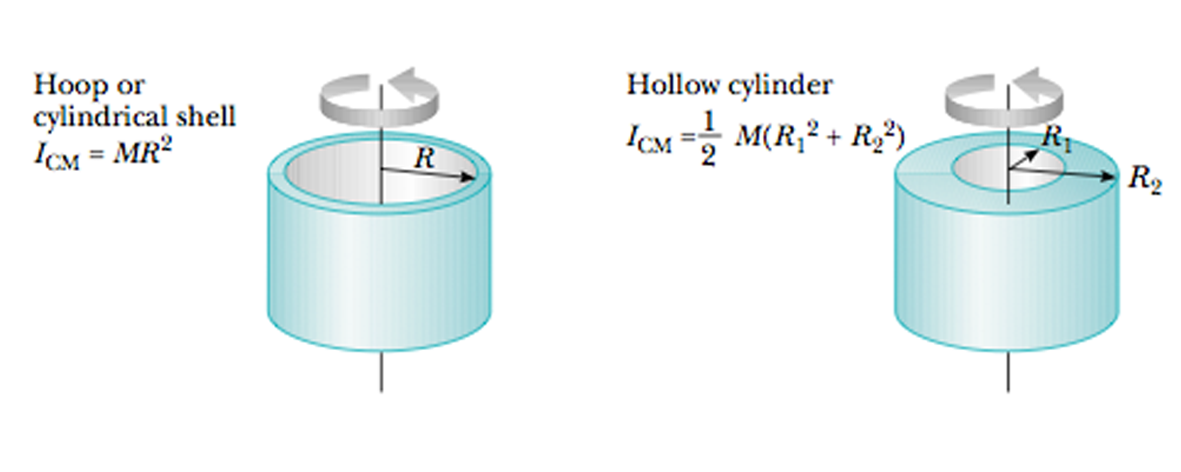
\includegraphics[width=13cm]{cmi1.png}}
\centerline{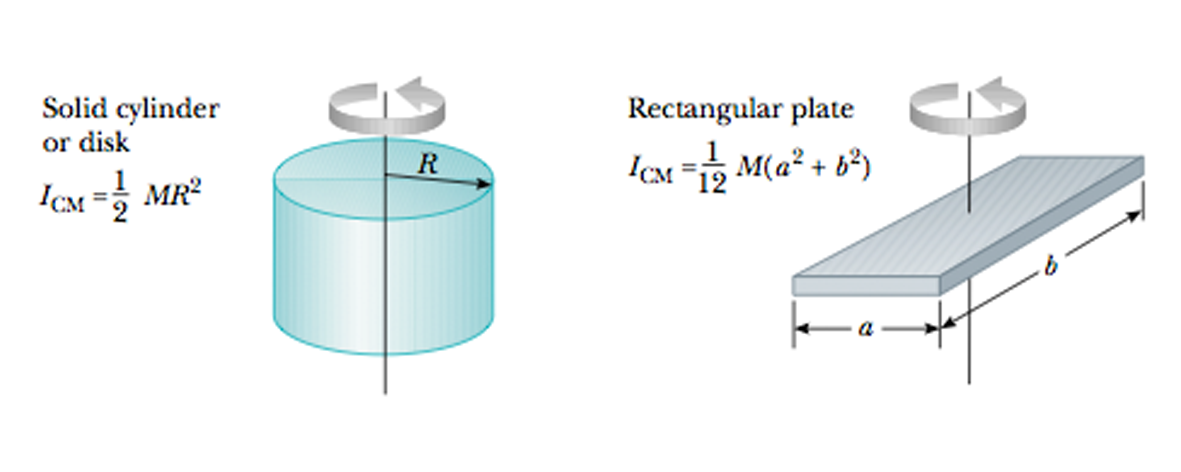
\includegraphics[width=13cm]{cmi2.png}}
\centerline{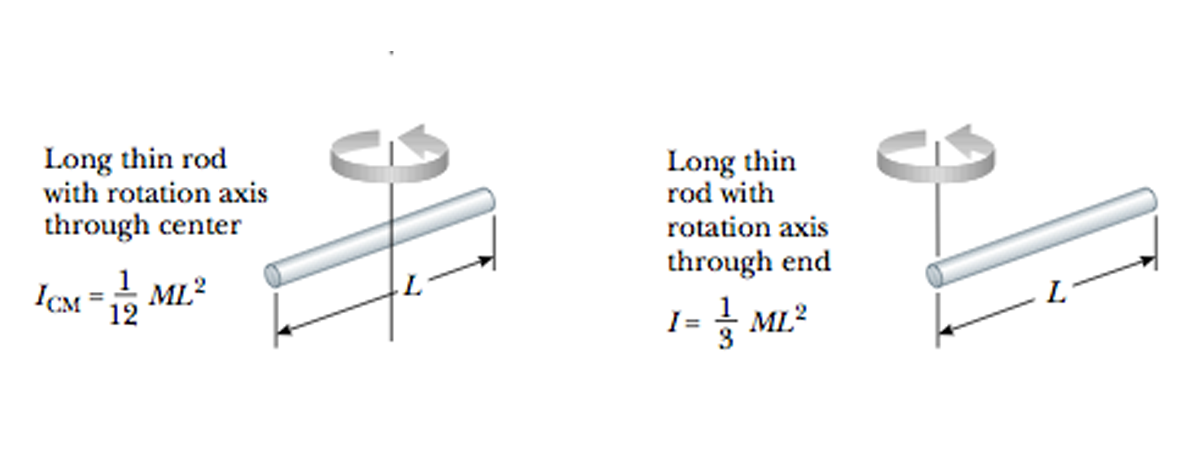
\includegraphics[width=13cm]{cmi3.png}}
\centerline{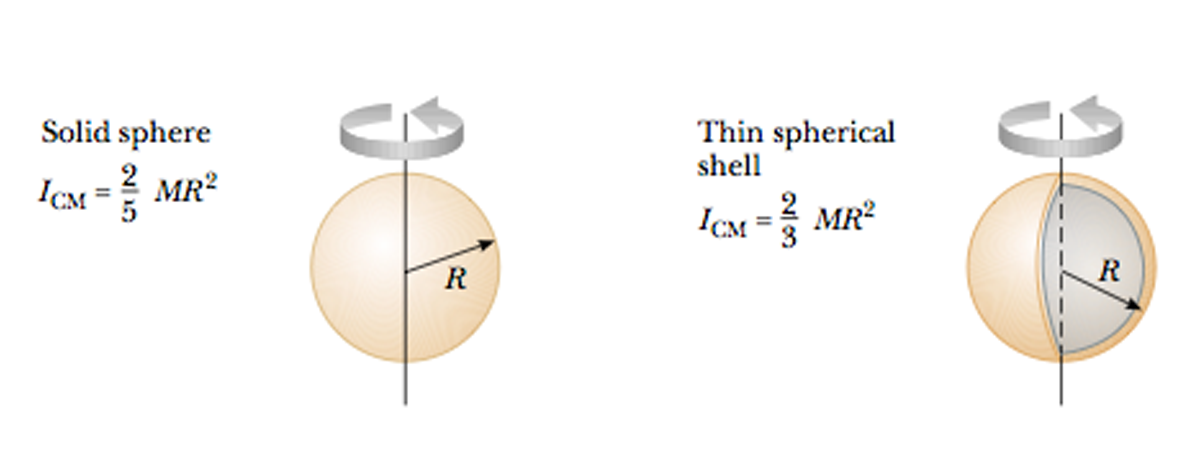
\includegraphics[width=13cm]{cmi4.png}}
\subsubsection{Parallel-Axis Theorem}
The calculation of moments of inertia about an arbitrary axis can be cumbersome, fortunately the parallel-axis theorem simplifies things. The parallel-axis theorem states that the moment of inertia about any axis parallel to and a distance $D$ away from this axis is:
\[
I=I_{CM}+MD^2
\]
\subsection{Torque}
The tendency of a force to rotate an object about some axis is measured by a vector quantity called \textbf{torque}, denoted by the symbol $\tau$. The applied force $\vec{F}$ acts at an angle $\phi$ to the horizontal. We define the magnitude of the torque associated with the force $\vec{F}$ by the expression:
\[
\tau=rF\sin(\phi)=Fd
\]
\ldots where $r$ is the distance between the pivot point and the point of application of $\vec{F}$ and $d$ is the perpendicular distance from the pivot point to the line of action of $\vec{F}$. (The line of action of a force is an imaginary line extending out both ends of the vector representing the force.) This quantity $d$ is called the moment arm (or lever arm) of $\vec{F}$.
\begin{multicols}{2}
  \centerline{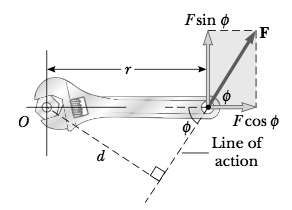
\includegraphics[width=5cm]{wrench.png}}
  \columnbreak
  The force $\vec{F}$ has a greater rotating tendency about $O$ as $F$ increases and as the moment arm $d$ increases. It is the component $F\sin(\phi)$ that tends to rotate the wrench about $O$. We use the convention that the sign of the torque resulting from a force is \textbf{positive} if the turning tendency of the force is counterclockwise and is \textbf{negative} if the turning tendency is clockwise.
\end{multicols}
the torque acting on the particle is proportional to its angular acceleration, and the proportionality constant is the moment of inertia. It is important to note that this is the rotational analog of Newton’s second law of motion, $\vec{F}=m\vec{a}$.
\[
\Sigma\tau=I\alpha
\]
Although each point on a rigid object rotating about a fixed axis may not experience the same force, linear acceleration, or linear speed, each point experiences the same angular acceleration and angular speed at any instant. Therefore, at any instant the rotating rigid object as a whole is characterized by specific values for angular acceleration, net torque, and angular speed.\\\\
Torque can also be expressed as the cross-product of $\vec{r}$ and $\vec{F}$, where it would be pointed perpendicular to their plane:
\[
\vec{\tau}=\vec{r}\times\vec{F}
\]
Right-hand rule: Hold your hands together, palm up, with the fingers curled. If the curl of your fingers represents a rotation from the first axis to the second, then the third axis points along your right thumb.

\subsection{Work, Power, and Energy in Rotational Motion}
The work done by $\vec{F}$ as the object rotates through an infinitesimal distance $ds=rd\theta$ in a time $dt$ is:
\[
dW=\vec{F}\cdot d\vec{s}=(F\sin(\phi))rd\theta
\]
where $F\sin(\phi)$ is the tangential component of $\vec{F}$, or, in other words, the component of the force along the displacement. Note that the radial component of F does no work because it is perpendicular to the displacement. Therefore we can see that:
\[
\frac{dW}{dt}=\tau\frac{d\theta}{dt} \indent
dW=\tau d\theta
\]
\[
W=\int_{\theta_i}^{\theta_f}\tau d\theta
\]
\[
\Sigma W=\frac{1}{2}I\omega_f^2-\frac{1}{2}I\omega_i^2
\]
\[
P=\frac{dW}{dt}=\tau\omega
\]

\subsection{Rolling Motion of a Rigid Object}
The linear speed and acceleration of the center of mass for pure rolling motion is given by (holds true whenever a cylinder or sphere rolls without slipping and is the condition for pure rolling):
\[
v_{CM}=\frac{ds}{dt}=R\omega
\]
\[
a_{CM}=\frac{dv_{CM}}=R\alpha
\]
We can express the total kinetic energy of the rolling cylinder as the equation below, where $I_P$ is the moment of inertia about a rotation axis through $P$.
\[
K=\frac{1}{2}I_P\omega^2 \indent
\text{\ldots apply parallel axis theorem} \indent
K=\frac{1}{2}I_{CM}\omega^2+\frac{1}{2}MR^2\omega^2=\frac{1}{2}I_{CM}\omega^2+\frac{1}{2}Mv_{CM}^2
\]
The total kinetic energy of a rolling object is the sum of the rotational kinetic energy about the center of mass and the linear kinetic energy of the center of mass.

\subsection{Angular Momentum}
The instantaneous angular momentum $\vec{L}$ of the particle relative to the origin $O$ is defined as the cross product of the particle’s instantaneous position vector $\vec{r}$ and its instantaneous linear momentum $\vec{p}$:
\[
\vec{L}=\vec{r}\times\vec{p}
\]
The net torque acting on a particle is equal to the time rate of change of the particle’s angular momentum:
\[
\Sigma\tau=\frac{d\vec{L}}{dt}
\]
\subsubsection{Conservation of Angular Momentum}
The total angular momentum of a system is constant in both magnitude and direction if the resultant external torque acting on the system is zero.
\[
\vec{L}_i=\vec{L}_f=constant
\]
\[
I_i\omega_i=I_f\omega_f
\]
The resultant torque acting on an object about an axis through the center of mass equals the time rate of change of angular momentum regardless of the motion of the center of mass.

\section{Equilibrium and Oscillation}
\subsection{Static Equilibrium}
Two forces $\vec{F}_1$ and $\vec{F}_2$ are equivalent if and only if $F_1=F_2$ and if and only if the two produce the same torque about any axis. In general, an object is in rotational equilibrium only if its angular acceleration $\alpha=0$. Because $\Sigma\tau=I\alpha$ for rotation about a fixed axis, our second necessary condition for equilibrium is that the net torque about any axis must be zero. We now have two necessary conditions for equilibrium of an object:
\[
\Sigma\vec{F}=0 \indent
\Sigma\vec{\tau}=0 \indent
\text{This is called \textbf{static equilibrium}}
\]
For a rigid body in static equilibrium the best way to solve for the unknown is to separate the forces into components, and set them equal to zero. The force of gravity exerted on an object can be considered as acting at a single point called the center of gravity. The center of gravity of an object coincides with its center of mass if the object is in a uniform gravitational field.

\subsection{Simple Harmonic Motion}
In general, a particle moving along the $x$-axis exhibits simple harmonic motion when $x$, the particle’s displacement from equilibrium, varies in time according to the relationship:
\[
x=A\cos(\omega t+\phi) \indent
\text{\ldots where $A$, $\omega$, and $\phi$ are constants}
\]
The period $T$ of the motion is the time it takes for the particle to go through one full cycle. We say that the particle has made one oscillation.
\[
T=\frac{2\pi}{\omega}
\]
The inverse of the period is called the frequency $f$ of the motion. The frequency represents the number of oscillations that the particle makes per unit time:
\[
f=\frac{1}{T}=\frac{\omega}{2\pi} \indent
\text{\ldots units are $s^{-1}$ or $Hz$}
\]
We can obtain the linear velocity of a particle undergoing simple harmonic motion by differentiating the position equation above:
\[
v=\frac{dx}{dt}=-A\omega\sin(\omega t+\phi)
\]
\[
a=\frac{dv}{dt}=-A\omega^2\cos(\omega t+\phi)
\]
Based on the fact that $x=A\cos(\omega t+\phi)$, we can simplify the expressions to find maximum values of speed and acceleration in simple harmonic motion:
\[
a_{max}=-\omega^2x
\]
\[
v_{max}=\omega A \indent
a_{max}=\omega^2A
\]
The following properties of a particle moving in simple harmonic motion are important:\\
\begin{enumerate}
\item The acceleration of the particle is proportional to the displacement but is in the opposite direction. This is the necessary and sufficient condition for simple harmonic motion, as opposed to all other kinds of vibration.
\item The displacement from the equilibrium position, velocity, and acceleration all vary sinusoidally with time but are not in phase.
\item The frequency and the period of the motion are independent of the amplitude.\\
\end{enumerate}
Whenever the force acting on a particle is linearly proportional to the displacement from some equilibrium position and in the opposite direction ($F=-kx$), the particle moves in simple harmonic motion. So we know that:
\[
a=-\frac{k}{m}x=-\omega^2x
\]
So, the frequency and period depend only on the mass of the block and on the force constant of the spring. Furthermore, the frequency and period are independent of the amplitude of the motion.
\[
T=\frac{2\pi}{\omega}=2\pi\sqrt{\frac{m}{k}} \indent
f=\frac{1}{T}=\frac{1}{2\pi}\sqrt{\frac{k}{m}}
\]
The total mechanical energy of a simple harmonic oscillator is a constant of the motion and is proportional to the square of the amplitude:
\[
E=\frac{1}{2}kA^2
\]
\centerline{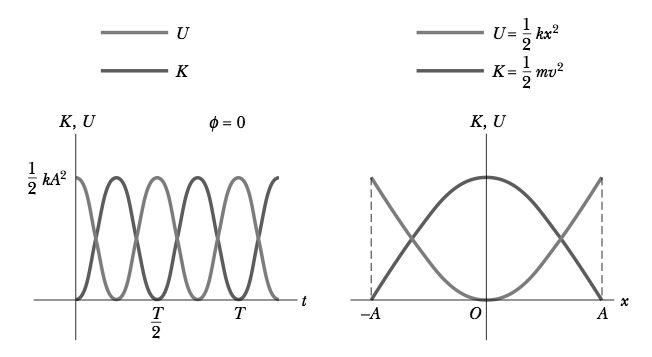
\includegraphics[width=14cm]{energyGr.png}}

\subsection{Simple Pendulum}
\begin{multicols}{2}
  The simple pendulum is another mechanical system that exhibits periodic motion. It consists of a particle-like bob of mass $m$ suspended by a light string of length $L$ that is fixed at the upper end, as shown in the figure on the right. Because $s=L\theta$ and $L$ is constant, we know that:
  \[
  \Sigma\vec{F}_t=-mg\sin(\theta)=m\frac{d^2s}{dt^2} \indent
  s=L\theta
  \]
  \[
  \frac{d^2\theta}{dt^2}=-\frac{g}{L}\sin(\theta)
  \]
  Now we assume that $\sin(\theta)\approx\theta$ (\textbf{small angle approximation}); thus the equation becomes:
  \[
  \frac{d^2\theta}{dt^2}=-\frac{g}{L}\theta
  \]
  \columnbreak
  \centerline{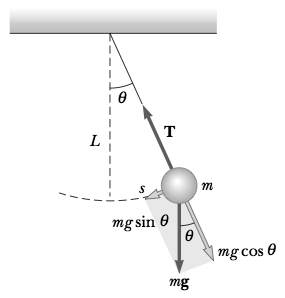
\includegraphics[width=5cm]{simPen.png}}
\end{multicols}
\[
\theta=\theta_{max}\cos(\omega t+\phi) \indent
\text{where $\theta_{max}$ is the maximum angular displacement and the angular frequency is $\omega=\sqrt{\frac{g}{L}}$}
\]
The period and frequency of a simple pendulum depend only on the length of the string and the acceleration due to gravity. Because the period is independent of the mass, we conclude that all simple pendulums that are of equal length and are at the same location (so that $g$ is constant) oscillate with the same period.
\[
T=2\pi\sqrt{\frac{L}{g}}
\]

\subsection{Physical Pendulum}
\begin{multicols}{2}
  If a hanging object oscillates about a fixed axis that does not pass through its center of mass and the object cannot be approximated as a point mass, we cannot treat the system as a simple pendulum. In this case the system is called a physical pendulum. The period of a physical pendulum can be calculated by:
  \[
  -mgd_{CM}\sin(\theta)=I\frac{d^2\theta}{dt^2}=-\omega^2\theta
  \]
  \[
  \omega=\sqrt{\frac{mgd_{CM}}{I}}
  \]
  \[
  T=\frac{2\pi}{\omega}=2\pi\sqrt{\frac{I}{mgd_{CM}}}
  \]        	\centerline{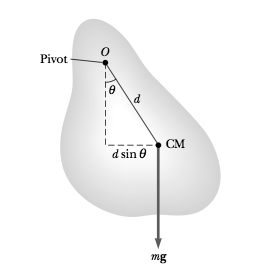
\includegraphics[width=5cm]{phyPen.png}}
\end{multicols}

\section{Electrostatics}
\subsection{Electric Charge}
There are two kinds of electric charges, positive and negative, and like charges repel one another and unlike charges attract one another. Another important aspect of Franklin’s model of electricity is the implication that electric charge is always conserved. $q$ is the common symbol for the charge. Therefore we conclude that electric charge has the following important properties:\\
\begin{enumerate}
\item Two kinds of charges occur in nature, with the property that unlike charges attract one another and like charges repel one another.
\item Charge is conserved.
\item Charge is quantized.
\end{enumerate}

\subsection{Conduction and Induction}
Electrical conductors are materials in which electric charges move freely, whereas electrical insulators are materials in which electric charges cannot move freely. Semiconductors are a third class of materials, and their electrical properties are somewhere between those of insulators and those of conductors. Silicon and germanium are well-known examples of semiconductors commonly used in the fabrication of a variety of electronic devices, such as transistors and light-emitting diodes.
\begin{multicols}{2}
  \centerline{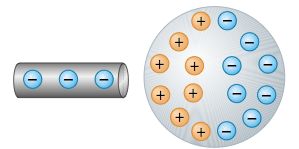
\includegraphics[width=5cm]{charges.png}}
  \columnbreak
  In this scenario the negatively rod charged is brought close to the neutral sphere, and as a result the electrons on the side closer to the rod were repelled. Thus, the negative rod induced a positive charge on the side of the rod.
\end{multicols}

\subsection{Coulomb's Law}
Charles Coulomb’s experiments in electrostatics showed that the electric force between two stationary charged particles is:\\
\begin{enumerate}
\item is inversely proportional to the square of the separation r between the particles and directed along the line joining them
\item is proportional to the product of the charges $q_1$ and $q_2$ on the two particles
\item is attractive if the charges are of opposite sign and repulsive if the charges have the same sign\\
\end{enumerate}
From these observations, we can express \textbf{Coulomb’s law} as an equation giving the magnitude of the electric force (sometimes called the \textit{Coulomb force}) between two point charges:
\[
\vec{F}_e=k_e\frac{\lvert q_1\rvert\lvert q_2\rvert}{r^2} \indent
\text{\ldots where $k_e$ is the Coulomb constant}
\]
\[
k_e=8.9875\times 10^9 \frac{Nm^2}{C^2}=\frac{1}{4\pi\epsilon_0}
\]
The smallest unit of charge known in nature is the charge on an electron or proton, which has an absolute value of:
\[
\lvert e \rvert = 1.602\times 10^{-19} C
\]

\subsection{Electric Field of Individual Charges}
The electric field $\vec{E}$ at a point in space is defined as the electric force $F_e$ acting on a positive test charge $q_0$ placed at that point divided by the magnitude of the test charge:
\[
\vec{E}=\frac{\vec{F_e}}{q_0}
\]
We say that an electric field exists at a point if a test charge at rest at that point experiences an electric force, but it can even exist at some point in empty space without a test charge. At any point $P$, the total electric field due to a group of charges equals the vector sum of the electric fields of the individual charges.

\subsection{Electric Field of a Continuous Charge}
To evaluate the electric field created by a continuous charge distribution, we use the following equation:
\[
\vec{E}=k_e\int\frac{dq}{r^2}\hat{r}
\]
It is usually easier to calculate electric fields in terms of the volume of the elements rather than their charge. So, we replace charge per unit length, area, or volume by symbols:
\[
\lambda=\frac{Q}{l} \indent
\sigma=\frac{Q}{A} \indent
\rho=\frac{Q}{V}
\]
If the charge is non-uniformly distributed over a volume, surface, or line, we have to express the charge densities as:
\[
\lambda=\frac{dQ}{dl} \indent
\sigma=\frac{dQ}{dA} \indent
\rho=\frac{dQ}{dV}
\]
where $dQ$ is the amount of charge in a small volume, surface, or length element.

\subsection{Electric Field Lines}
Electric field lines are a convenient way of visualizing electric field patterns, and are related to the electric field in any region of space in the following manner:\\
\begin{itemize}
\item The electric field vector $\vec{E}$ is tangent to the electric field line at each point
\item The number of lines per unit area through a surface perpendicular to the lines is proportional to the magnitude of the electric field in that region. Thus, $E$ is great when the field lines are close together and small when they are far apart.\\
\end{itemize}
\begin{multicols}{2}
  The rules for drawing electric field lines are as follows:\\
  \begin{itemize}
  \item The lines must begin on a positive charge and terminate on a negative charge
  \item The number of lines drawn leaving a positive charge or approaching a negative charge is proportional to the magnitude of the charge
  \item No two field lines can cross
  \end{itemize}
  \vfill
  \columnbreak
  \centerline{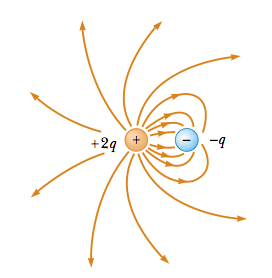
\includegraphics[width=4cm]{fieldLines.png}}
\end{multicols}

\subsection{Motion of a Charged Particle}
After applying Newton's Second Law $\vec{F}=m\vec{a}$, we can solve for the acceleration of the particle:
\[
\vec{F}_e=q\vec{E}=m\vec{a}
\]
\[
\vec{a}=\frac{q\vec{E}}{m}
\]
If $\vec{E}$ is uniform (that is, constant in magnitude and direction), then the acceleration is constant. If the particle has a positive charge, then its acceleration is in the direction of the electric field. If the particle has a negative charge, then its acceleration is in the direction opposite the electric field.

\section{Electric Flux and Potential}
\subsection{Electric Flux}
The number of electric field lines per unit area is proportional to the magnitude of the electric field, and this can be written as the total number of lines penetrating the surface is proportional to the product $EA$, this is Electric Flux. Electric flux is proportional to the number of electric field lines penetrating some surface:
\[
\Phi_E=EA \indent\frac{Nm^2}{C}
\]
If we let the area of each element approach zero, then the number of elements approaches infinity and the sum is replaced by an in- tegral. Therefore, the general definition of electric flux is:
\[
\Phi_E=\underset{surface}{\oint}\vec{E}\cdot d\vec{A}
\]

\subsection{Gauss's Law}
There exists a general relationship between the net electric flux through a closed surface (often called a \textit{gaussian surface}) and the charge enclosed by the surface. This relationship, known as Gauss’s law, is of fundamental importance in the study of electric fields. Let us again consider a positive point charge q located at the center of a sphere of radius $r$.
\begin{multicols}{2}
  \centerline{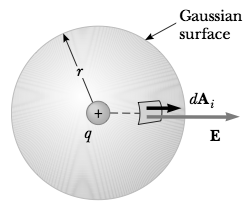
\includegraphics[width=4cm]{gaussLaw.png}}
  \columnbreak
  \[
  \Phi_E=\oint\vec{E}\cdot d\vec{A}=\vec{E}\oint dA
  \]
  \[
  \Phi_E=\frac{k_eq}{r^2}(4\pi r^2)=4\pi k_eq \indent
  k_e=\frac{1}{4\pi\epsilon_0}
  \]
  \[
  \Phi_E=\frac{q_{enc}}{\epsilon_0}
  \]
\end{multicols}
If there is a charge outside a sphere the number of electric field lines entering the surface equals the number leaving the surface. Therefore, we conclude that the net electric flux through a closed surface that surrounds no charge is zero. \textbf{Gauss’s law}, which is a generalization of what we have just described, states that the net flux through any closed surface is:
\[
\Phi_E=\oint\vec{E}\cdot d\vec{A}=\frac{q_{enc}}{\epsilon_0}
\]

\end{document}


































